
\documentclass{article}
\usepackage[utf8]{inputenc}
\usepackage[spanish]{babel}
\usepackage{amsmath, amsthm, amsfonts}
\usepackage{multicol}
\usepackage{graphicx}
\usepackage{vmargin}
\setmargins{2.5cm}       % margen izquierdo
{1.5cm}                        % margen superior
{16.5cm}                      % anchura del texto
{23.42cm}                    % altura del texto
{10pt}                           % altura de los encabezados
{1cm}                           % espacio entre el texto y los encabezados
{0pt}                             % altura del pie de página
{2cm}                           % espacio entre el texto y el pie de página

\newtheorem{thm}{Teorema}[section]
\newtheorem{cor}[thm]{Corolario}
\newtheorem{lem}[thm]{Lema}
\newtheorem{prop}[thm]{Proposición}
\theoremstyle{definition}
\newtheorem{defn}[thm]{Definición}
\theoremstyle{remark}
\newtheorem{rem}[thm]{Observación}
\def\RR{\mathbb{R}}
\def\ZZ{\mathbb{Z}}
\newcommand{\abs}[1]{\left\vert#1\right\vert}
\usepackage{stackrel}

%--------------------------------------------------------------------------
\DeclareMathOperator{\Jac}{Jac}

%--------------------------------------------------------------------------
\title{Cadenas de Markov}

\author{
	Calixtro Ames, Cynthia Lizeth\\
	\texttt{ccalixtroa@uni.pe}\\
	\small{Escuela de Ciencia de la Computación}\\
	\small{Universidad Nacional de Ingeniería}
	\and
	Huamaní Inga, Alex Raúl\\
	\texttt{ahuamanii@uni.pe}\\
	\small{Escuela de Matemática}\\
	\small{Universidad Nacional de Ingeniería}
}

\begin{document}
\maketitle

\abstract{Aquí va el resumen}

\section{Introducción}
\subsection{Conceptos previos}
\subsubsection{Procesos Estocásticos}\label{sec:nada}

Un proceso estocástico se puede definir equivalentemente de dos formas diferentes:\\

1. Como un conjunto de realizaciones temporales y un índice aleatorio que selecciona una de ellas.\

2. Como un conjunto de variables aleatorias $X_{t}$ indexadas por un índice $t$ , dado que $t \in T$ con $T\subseteq \mathbb{R} $.
\\\

Un proceso se dice de \textbf{tiempo continuo} si $T$ es un intervalo (usualmente este intervalo se toma como $[0,\infty\rangle$) o de \textbf{tiempo discreto} si $T$ es un conjunto numerable (solamente puede asumir determinados valores, usualmente se toma $T \subseteq \mathbb{N}$). De donde el conjunto $T$ sera llamado \textbf{espacio parametral} en donde las variables aleatorias toman valores en un conjunto $S$ llamado \textbf{espacio de estados}

\subsubsection{Trayectoria de un proceso}\label{sec:nada2}
Una $trayectoria$ de un proceso estocástico $x_{t}: t \in T$ es una función $$t \longmapsto X_{t}(w)]$$ para cada $w \in \omega.$
\ Existen distintos tipos de procesos estocásticos. Éstos se obtienen al considerar 
\begin{itemize}
	\item Distintos espacios parametrales.
	\item Distintos espacios de estado.
	\item Distintas características de la trayectorias.
	\item Distintas relaciones de dependencia estocástica entre las variables aleatorias que conforman el proceso.
\end{itemize}
\subsubsection{Algunos ejemplos de procesos}
\begin{itemize}
	\item \textbf{Proceso de ensayos independientes}\\
	supongamos que el espacio parametral $T={1,2,\dots}$ es el conjunto de numeros naturales y $S \subseteq \mathbb{R}$, cuando las variables aleatorias$(X_{1},X_{2},\dots)$ son independientes se dice que este es un proceso estocastico de
	ensayos independientes, "recordar que una coleccion infinita de variables es independientes si toda subcoleccion finita lo es" \\
	\item \textbf{Procesos de Markov} \\
	El proceso ${X_{t}: t=0,1,\dots}$ es donde $X_{t} \in S$ es discreto es un \textbf{proceso de Markov} si para cada $x_0,x_1,\dots,x_{n+1} en S$ se cumple la siguiente propiedad 
	$$ P(X_{n+1}=x_{n+1}|X_0=x_0,\dots,X_n=x_n)=P(X_{n+1}=x_{n+1}|X_{n}=x_n) $$
	Es decir la historia del proceso hasta el tiempo n-1 es irrelevante cuando se conoce el estado del proceso al tiempo $n$ a esta identidad se le conoce con el nombre de \textbf{propiedad de Markov} y es un buen ejemplo del tipo de 
	dependencia estocástica que puede existir entre las variables de un proceso en este caso las variables aleatorias son discretas y al proceso lo llamaremos \textbf{Cadenas de Markov} en este pequeño articulo nos centraremos en esto. \\
	\item \textbf{Procesos con incrementos independientes} \\
	el proceso $ {X_{t}: t \geq 0}$ tiene \textbf{incrementos independientes} si las variables aleatorias $$X_{t1},X_{t2}-X_{t1},\dots, X_{tn}- X{tn-1}$$ son independientes para cualesquiera tiempos  $0\leq t_{1}<t_{2}<\dots<t_{n}.$\\
	\item \textbf{Procesos estacionarios}\\
	El proceso ${X_{t}:t\geq0}$ es \textbf{estacionario} en el sentido estricto si para cualesquiera $t_1,\dots,t_n,h \geq 0$
	$$(X_{t_1},\dots,X_{t_n})\stackrel{d}{=}(X_{t_1+h},\dots,X_{t_n+h})$$
	de donde el vector aleatorio del lado derecho tiene la misma distribucion que el vector aleatorio del lado izquierdo. Esto significa que el vector aleatorio del lado izquierdo se puede trasladar en el tiempo como indica el vector del lado derecho sin que cambie su distribucion de probabilidad.\\
	\item \textbf{Procesos con incrementos estacionarios}\\
	El proceso ${X_t : t \geq 0}$ tiene \textbf{incrementos estacionarios} si para cualesquiera $0\leq S < t; h \geq 0 $ $$X_t - X_s \stackrel{d}{=} X_{t+h} - X_{s+h} $$
	\item \textbf{Martingalas} \\
	El proceso ${X_t : t = 0,1,\dots}$ es una \textbf{Martingala} si $$E(X_{n+1}|X_0=x_0,\dots,X_n=x_n)=x_n$$ pero en realidad hay otras condiciones tecnicas que se piden a un proceso para que sea un martingala.\\
	\item Procesos de Lévy \\
	El procese ${X_t: t\geq0}$ es un \textbf{proceso de Lévy} si sus incrementos son:
	\begin{itemize}
		\item Independientes
		\item Estacionarios
	\end{itemize}
	\item \textbf{Procesos Gausianos}\\
	El proceso $X_t: t\geq 0$ es un \textbf{proceso gausiano} si para cualesquiera tiempos $t_1,\dots,t_n$ 
	$$(X_{t_1},\dots,X_{t_n}) \sim \mbox{Normal multivariada}$$
\end{itemize}

Observaciones. No debe pensarse que estas caracteristicas de los procesos son excluyentes unas de otras, por ejemplo existen varios procesos estocasticos que cumplen varias de estas propiedades al mismo tiempo, por ejemplo el movimiento Browmiano es un proceso estocastico importante es un proceso \textbf{gausiano} con \textbf{incrementos independientes} y \textbf{estacionarios} por lo tanto es un proceso de \textbf{Lévy}, puede ademas demostrarse que es una \textbf{Martingala} y  que cumple la \textbf{propiedad de Markov}

\subsection{Conceptos y simulación}
\subsubsection{Cadenas de Markov}
\textbf{Definición 1. Espacio de estados}\\
Definimos el \textit{espacio de estados} como el conjunto formado por todos los posibles valores que puede tomar $X_{n}$ donde el índice $n$ representa la evolución del proceso en el \textit{tiempo}. Para una cadena de Markov tanto el \textit{espacio de estados} como el \textit{tiempo} pueden ser discreto o continuo.\\

\textbf{Definición 2. Cadena de Markov}\\
Una cadena de Markov es una secuencia de variables aleatorias $X_{0},X_{1},X_{2},...$ que toman valores en en \textit{espacio de estados} $\{1,2,\dots,M\}$ si para todo $n\geq0$ se cumple la propiedad de Markov. Donde $P(X_{n+1}=x_{n+1}|X_{n}=x_n)$ se denomina probabilidad de transición desde el estado $i$ hacia el estado $j$. Como esta probabilidad no depende de el valor de $n$ se dice que el tiempo es \textit{homogeneo}.\\

\textbf{Definición 3. Matriz de transición}\\
Sean $X_{0},X{1},X_{2},\dots$ una cadena de Markov con espacio de estados $\{1,2,\dots,M\}$ y sea
\[
p_{ij} = P(X_{n+1}=j|X_{n}=i)
\] 
la probabilidad de transición del estado $i$ al estado $j$. Entonces, a la matriz $M$x$M$, $P$ = $\{p_{ij}\}$ se le denomina \textit{matriz de transición} de la cadena. Además, la suma de los valores por fila es igual a 1.\\

\textbf{Definición 4. Propabilidad de transición en n pasos}
La probabilidad de transición en $n$ pasos de $i$ hacia $j$ es la probabilidad de ir de $i$ hacia $j$ en $n$ pasos. Denotamos esto como $p_{ij}^{(n)}$ y se define de la siguiente manera:
\[
p_{ij}^{(n)} = P(X_{n}=j|X_{0}=i)
\]
y se cumple que $p_{ij}^{(n)}$ es el elemento de subíndices $(i,j)$ de la matriz $P^{n}$\\

\textbf{Definición 5. Distribución Marginal de $X_{n}$}\\
Sea el vector fila $q = (q_{1},\dots,q_{M})$ con $q_{i} = P(X_{0} = i)$ entonces la \textit{distribución marginal} de $X_{n}$ está dada por el vector $qP^{n}$. Es decir, el $j$-ésimo componente del vector $qP^{n}$ es $P(X_{n} = j)$
\subsubsection{Cadena de Markov Irreductible}
Se dice que una cadena de Markov con matriz de transición $P$ es \textit{irreductible} si para dos estados $i$ y $j$ cualesquiera existe un entero positivo $n$ tal que el elemento de índices $(i,j)$ en la matriz $P^n$ es positivo. Es decir, es posible ir de $i$ a $j$ en un número finito de pasos. En caso contrario se dirá que la cadena de Markov es \textit{reducible}.

\subsubsection{Cadena de Markov Periódica}
\textbf{Definición 6. Periodo de un estado}\\
Se define el periodo $d_{i}$ de el estado $i$ como
\[
d_{i} = gcd\{n\geq1:p_{ii}^{(n)}>0\}
\]
Esto es, el \textit{gcd} (\textit{máximo común divisor}) del posible número de pasos que puede tomar para regresar al mismo estado, en este caso, al estado $i$. 
Cuando un estado tiene periodo igual a 1 entonces se dirá que es \textit{aperiódico}, en caso contrario, se le llamará \textit{periódico}.\\

Una cadena de Markov es llamada \textit{aperiódica} cuando todos sus estados son aperiódicos. En caso contrario, se le denomina \textit{periódica}.

\subsubsection{Distribuciones estacionarias}
Un vector fila $\pi$ = $(\pi_{1},\dots,\pi_{M})$ con $\pi_{i}\geq0$ and $\sum_{i}\pi_{i} = 1$ es una \textit{distribución estacionaria} para una cadena de Markov con \textit{matriz de transición} $P$ si
\[
\pi P = \pi
\]
Si $\pi$ es la distribución de $X_{0}$, esto es si $\pi_{i} = P(X_{0} = i)$, entonces $\pi P$ vendría a ser la distribución marginal de $X_{1}$. Esto significa que, si $X_{0}$ tiene distribución $\pi$, entonces $X_{1}$ también tendrá una distribución $\pi$. Si $X_{2}$ tiene una distribución $\pi$ entonces $X_{3}$ también la tendrá y así sucesivamente.
Por lo tanto, una distribución estacionaria de una cadena de Markov es una distribución de probabilidad que se mantiene sin cambios en la cadena a medida que avanza el tiempo.
\subsubsection{Simulaciones}
\textbf{A. Simulación de una cadena de Markov}

\begin{figure}[!h]
	\centering
	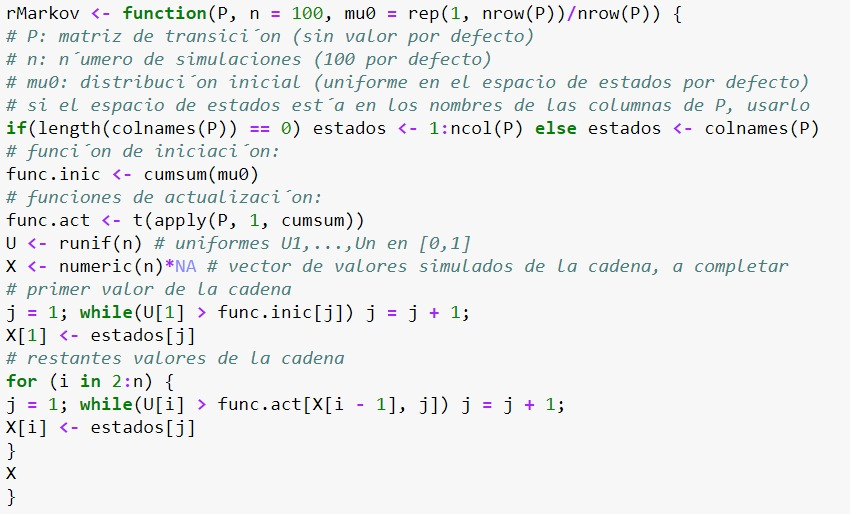
\includegraphics[scale=0.8]{fun1}
	\caption{Función que simula una cada de Markov.}
	\label{figura1}
\end{figure}

Si consideramos un espacio de estados $E=\{A,C,G,T\}$ (A=adenina,C=citosina,G=guanina,T=timina)

\begin{figure}[!h]
	\centering
	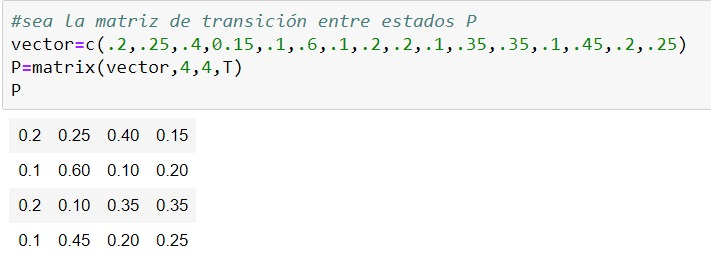
\includegraphics[scale=0.8]{fun2}
	\caption{Matriz de transición de la cadena de Markov.}
	\label{figura2}
\end{figure}

\begin{figure}[!h]
	\centering
	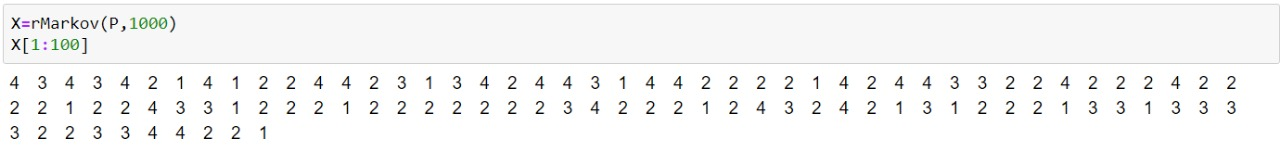
\includegraphics[scale=0.55]{fun3}
	\caption{Probando la función \textit{rMarkov}.}
	\label{figura3}
\end{figure}

\begin{figure}[!h]
	\centering
	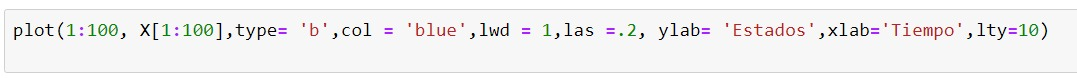
\includegraphics[scale=0.7]{fun4}
	\caption{Graficando la cadena de Markov.}
	\label{figura4}
\end{figure}

\begin{figure}[!h]
	\centering
	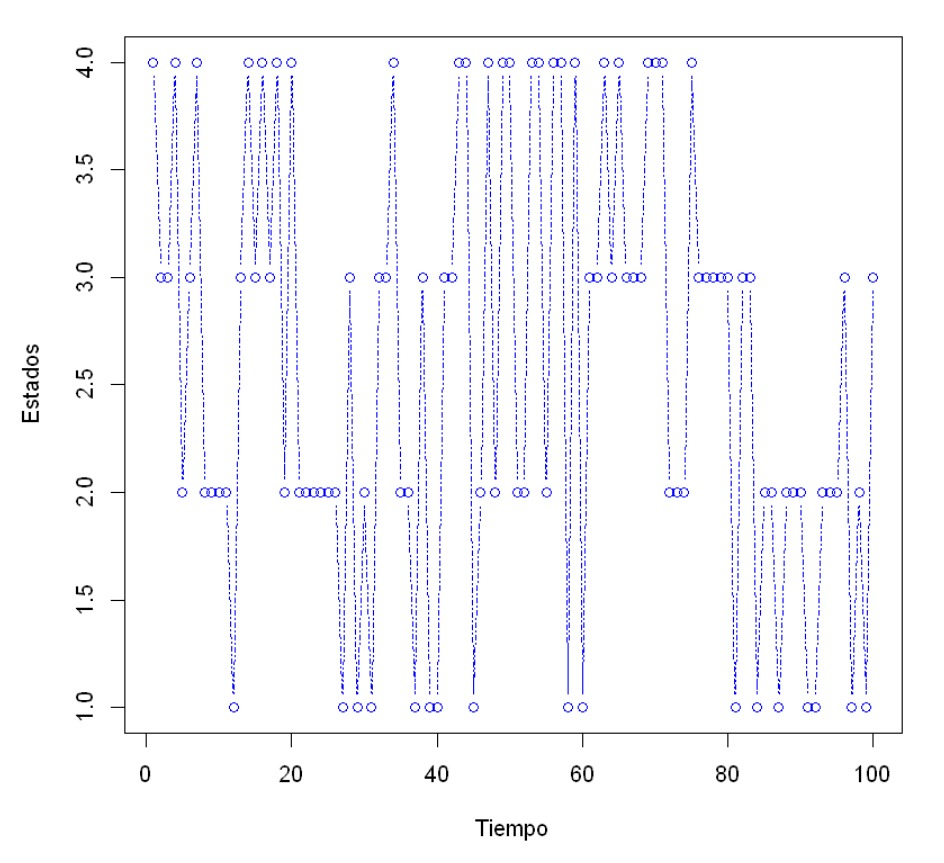
\includegraphics[scale=0.9]{fun5}
	\caption{Grafica Tiempo VS Estados.}
	\label{figura5}
\end{figure}

\begin{thebibliography}{99}

\bibitem{Cd94} Autor, \emph{Ttulo}, Revista/Editor, (ao)

\end{thebibliography}

\end{document}